\chapter{Представление данных в вычислительных системах}



\section{Представление целочисленных данных}

В этом разделе описываются два разных способа использования битов для представления целых чисел: один из этих способов позволяет представлять только неотрицательные числа, а другой --- отрицательные числа, положительные и ноль. Позже мы увидим, что они сильно взаимосвязаны как математическими свойствами, так и реализациями на машинном уровне. Мы также рассмотрим влияние расширения или сжатия целых чисел, чтобы их можно было уместить в представления с разной длиной.

\subsection{Представление целых без знака}

Пусть имеется целочисленный тип, представляющий значения из w бит. Битовый вектор записывается либо как $\vec{x}$, что обозначает вектор как единое целое, либо как $[x_{n-1}, x_{n-2}...x_0]$ с перечислением отдельных битов в векторе. Рассмотрим $\vec{x}$ как число, записанное в двоичном виде. В этом случае мы получим интерпретацию $\vec{x}$ как числа без знака. Каждый бит $x_i$ имеет значение 0 или 1. В последнем случае он соответствует величине $2^i$, которая является составной частью всего числа.



\section{Представление значений с плавающей точкой. Cтандарт IEEE}

Позиционное представление, подобное рассмотренному в предыдущем разделе, неэффективно для очень больших чисел. Например, представление $5 × 2^{100}$ будет состоять из комбинации битов 101, за которой следует 100 нулей. Вместо этого предпочтительнее представлять такие числа в форме $x × 2^y$ путем задания значений х и y.

Стандарт IEEE определяет представление чисел с плавающей точкой в виде:
\begin{center}
    \large{$V = (-1)^s × M × 2^E$}
\end{center}
где:
\begin{itemize}
    \item символ $s$ определяет знак числа, который может быть отрицательным при $s = 1$ или положительным при $s = 0$ (интерпретация знакового разряда для числового значения 0 рассматривается как особый случай);
    \item мантисса М --- дробное двоичное число в диапазоне от 1 до 2 – $\varepsilon$ или от 0  до 1 – $\varepsilon$ (значение $\varepsilon$ определяет точность вычислений и зависит от разрядности мантиссы);
    \item показатель Е – взвешивает величину (возможно, отрицательной)  степенью 2.
\end{itemize}

Для кодировки этих величин битовое представление числа с плавающей точкой делится на три поля:

\begin{itemize}
    \item знаковый бит s напрямую кодирует символ s;
    \item k-разрядное поле показателя $ехр = e_{k-1} ... e_1e_0$ кодирует показатель Е;
    \item n-разрядное поле дробной части $frac = f_{n-1} ... f_1f_0$ кодирует мантиссу М, способ кодирования также зависит от того, равно поле показателя 0 или нет.
\end{itemize}

На рис~\ref{data01}. 2.13 показано, как эти три поля упакованы в два наиболее распространенных формата. В формате с одинарной точностью (тип float в языке С) поля s, exp и frac имеют размеры 1, k = 8 и n = 23 бит, что дает 32-разрядное представление. В формате с двойной точностью (тип double в языке С) поля s, ехр и frac имеют размеры 1, k = 11, n = 52 бит, что дает 64-разрядное представление.

\begin{figure}[htbp]
    \centering
    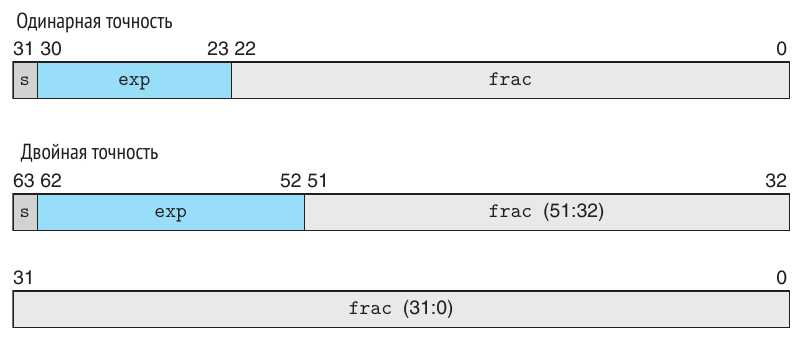
\includegraphics[width=0.8\textwidth]{img/data01.png}
    \caption{Стандартные форматы представления чисел с плавающей запятой}
    \label{data01}
\end{figure}

Величину, представленную конкретным битовым представлением, можно разделить на три разных варианта (последний имеет два подварианта), в зависимости от значения ехр. Они показаны на рисунке~\ref{data02}.

\begin{figure}[htbp]
    \centering
    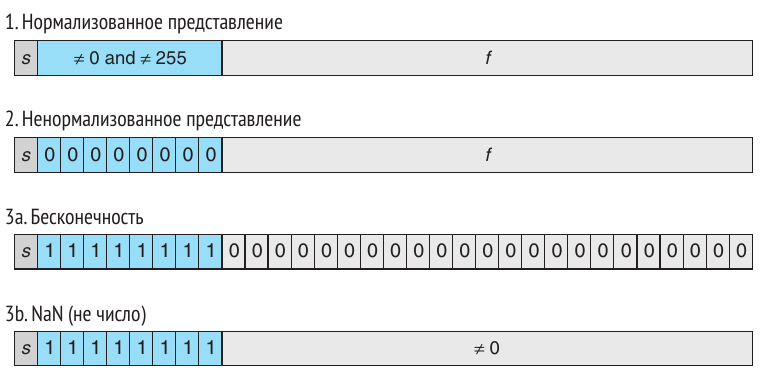
\includegraphics[width=0.8\textwidth]{img/data02.png}
    \caption{Категории значений с плавающей запятой одинарной точности. Значение показателя определяет, является число (1) нормализованным, (2) ненормализованным или (3) особым}
    \label{data02}
\end{figure}

\subsection{Вариант 1: нормализованные значения}

Это самый общий случай. Он имеет место, когда комбинация битов ехр состоит либо из одних нулей (числовое значение 0), либо из одних единиц (числовое значение 255 для одинарной точности и 2047 для двойной). В этом случае поле показателя интерпретируется как целое со знаком в смещенной форме. То есть показатель имеет значение $Е = е - Bias$ (смещение), где $е$ – число без знака с битовым представлением $e_{k-1} ... e_1e_0$, a $Bias$ --- величина смещения, равная $2^{k-1} - 1$ (127 для одинарной точности, 1023 --- для двойной). Это разложение дает диапазон показателей от -126 до +127 для одинарной точности и от -1022 до +1023 – для двойной.

Поле дробной части frac интерпретируется как представляющее дробную величину f, где $0 \leq f < 1$, имеющую двоичное представление $0.f_{n-1} ... f_1f_0$, т.~ е. с двоичной точкой слева от самого значимого бита. Мантисса определяется как $М = 1 + f$. Иногда такое представление называют представлением с неявной ведущей единицей, потому что M можно рассматривать как число с двоичным представлением $1.f_{n-1}f{n-2} ... f_0$. Такое представление позволяет получить дополнительный бит точности, поскольку показатель Е всегда можно настроить так, чтобы мантисса М находилась в диапазоне $1 \leq M < 2$ (при условии отсутствия переполнения). Поэтому нет необходимости явно представлять ведущий, так как он всегда равен единице.

\begin{center}
\framebox[\textwidth][l]{
\begin{minipage}{0.95\linewidth}
\textbf{Зачем устанавливать смещение для ненормализованных значений}

Использование значения показателя 1 - Bias вместо простого -Bias может показаться противоречащим здравому смыслу. Но очень скоро вы увидите, что такое представление упрощает переход от ненормализованных значений к нормализованным.
\end{minipage}
}
\end{center}

\subsection{Вариант 2: ненормализованные значения}

Когда поле показателя состоит только из нулей, то представляемое число находится
в ненормализованной форме. В этом случае значение порядка Е = 1 - Bias, а значение мантиссы M = f, т. е. значение дробной части не имеет неявной ведущей единицы.

Ненормализованные значения служат двум целям. Во-первых, они позволяют представлять числовое значение 0, поскольку для нормализованного представления всегда выполняется условие $M \geq 1$, и, следовательно, оно не позволяет представить 0. Фактически представление чисел с плавающей точкой +0.0 имеет комбинацию битов, состоящую из одних нулей: знаковый разряд содержит 0, поле показателя
полностью состоит из нулей (что указывает на ненормализованное значение), и поле дробной части тоже состоит из одних нулей, давая M = f = 0. Интересно, что когда знаковый разряд равен единице, а все другие поля – нулю, то получается значение -0.0. В формате IEEE с плавающей точкой значения -0.0 и +0.0 в одних случаях
рассматриваются как разные, а в других – как одинаковые.

Вторая цель, которую преследуют ненормализованные значения, – представление чисел, близких к 0.0. Они обеспечивают свойство равномерного приближения к нулю, при котором возможные числовые значения равномерно располагаются около 0.0.

\subsection{Вариант 3: особые значения}

Последняя форма представления значений используется, когда поле показателя со
стоит из одних единиц. Если при этом поле дробной части состоит из одних нулей, то в результате получается бесконечность: либо $+\infty$, когда s = 0, либо $-\infty$, когда s = 1. Бесконечность может представлять переполнение как при умножении очень больших чисел, так и при делении на ноль. Когда дробная часть не равна нулю, то такое значение называется NaN (сокращенно <<Not a Number>> – не число). Такие значения возвращаются, когда результат операции нельзя представить вещественным числом или бесконечностью, как, например, $\sqrt{-1}$ или $\infty - \infty$. Они также могут пригодиться в некоторых приложениях для инициализации данных.
